\documentclass[13pt]{article}
\usepackage{amsmath, amsthm, amssymb, graphicx, enumitem, esvect}


% Language setting
% Replace `english' with e.g. `spanish' to change the document language
\usepackage[english]{babel}

% Set page size and margins
% Replace `letterpaper' with `a4paper' for UK/EU standard size
\usepackage[letterpaper,top=2cm,bottom=2cm,left=3cm,right=3cm,marginparwidth=1.75cm]{geometry}

\title{C\&EE 110 Homework 4}
\author{Warren Kim}

\begin{document}
\maketitle

\newpage
\section*{Problem 1}
\begin{enumerate}[label=(\alph*)]
\item Y has a \textbf{hypergeometric probability distribution} since
  we remove elements from the sample size without replacing them.
\item \[P(Y = y) = \frac{ {5 \choose y } { 5 \choose {4 - y} } }{ { 10
        \choose 4 } }, \ y = 0, 1, 2, 3, 4\] 
  \begin{center}
    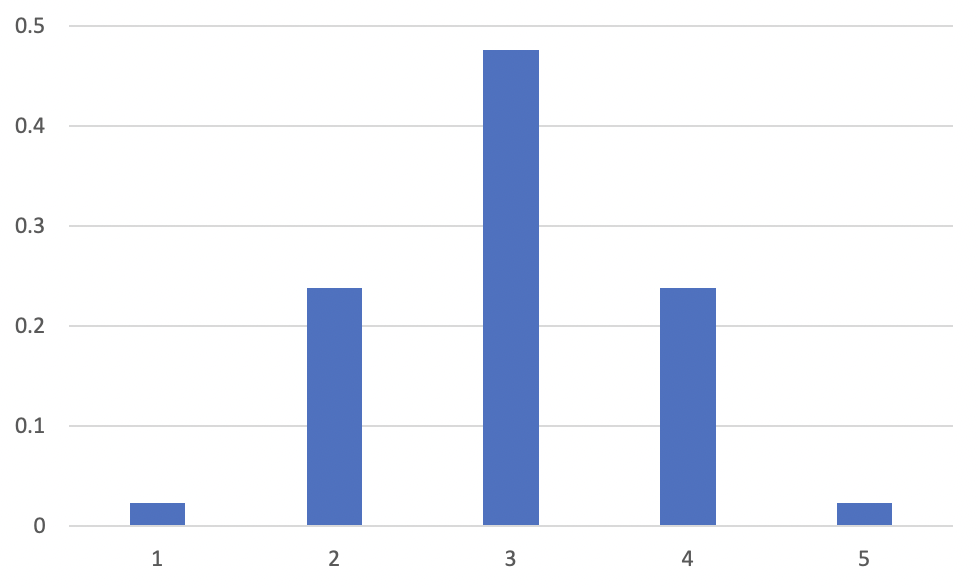
\includegraphics[scale=0.5]{images/hypergeo.png}
    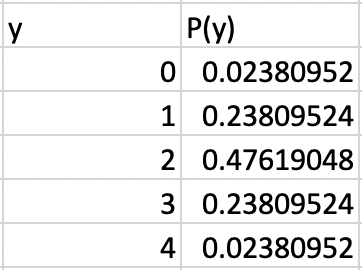
\includegraphics[scale=1]{images/table.png}
  \end{center}
\item \[P(Y \geq 2) = \sum_{y = 2}^{4} P(y) = 0.738\]
\end{enumerate}

\newpage
\section*{Problem 2}
\begin{enumerate}[label=(\alph*)]
\item
  \begin{align*}
    p(y) &= \frac{\lambda^{y}}{y!}e^{-\lambda} && \lambda = 5 \cdot 2 =
                                                  10, \ y \leq 6 \\
         &= \sum_{y = 0}^{6} \frac{10^{y}}{y!}e^{-10} \\
    p(y) &= 0.130
  \end{align*}

\item
  \begin{align*}
    p(y) &= \frac{\lambda^{y}}{y!}e^{-\lambda} && \lambda = 5, \ y < 3 \\
         &= \sum_{y = 0}^{2} \frac{10^{y}}{y!}e^{-10} \\
    p(y) &= 0.125
  \end{align*}
  
\item \[m(t) = \bigg(\frac{1}{6}\bigg)e^{t} +
    \bigg(\frac{2}{6}\bigg)e^{2t} + \bigg(\frac{3}{6}\bigg)e^{3t}\]
  \begin{enumerate}[label=(\textit{\roman*})]
  \item \[E(Y) = m'(0) = \bigg(\frac{1}{6}\bigg)e^{t} +
      \bigg(\frac{4}{6}\bigg)e^{2t} + \bigg(\frac{9}{6}\bigg)e^{3t} = \frac{7}{3}\]
  \item
    \begin{align*}
      V(Y) &= E'(Y^{2}) - [E(Y)]^{2} \\
           &= m''(0) - [m'(0)]^{2} \\
           &= \bigg[\bigg(\frac{1}{6}\bigg)e^{t} +
             \bigg(\frac{8}{6}\bigg)e^{2t} +
             \bigg(\frac{27}{6}\bigg)e^{3t}\bigg] -
             \bigg[\frac{7}{3}\bigg]^2 \\
      V(Y) &= \frac{5}{9}
    \end{align*}
  \item
    \begin{align*}
      m(t) &= E(e^{tY}) \\
           &= \sum_{y}  e^{ty}p(y) \\
             &= \frac{1}{6}e^{t} + \frac{2}{6}e^{2t} +
               \frac{3}{6}e^{3t} \\
           &= \sum_{y} [1 + 2e^t + 3e^{2t} + \ldots] \frac{1}{6}e^{t}
    \end{align*}
    \begin{center}
      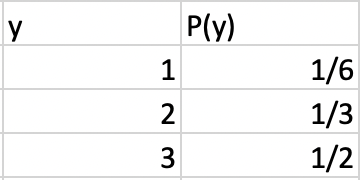
\includegraphics[scale=1]{images/fractions.png}
    \end{center}    
  \end{enumerate}
\end{enumerate}

\newpage
\section*{Problem 3}
\begin{enumerate}[label=(\alph*)]
\item
  \begin{align*}
    1 &= \int_{0}^{\infty} ce^{-4x}dx \\
      &= \frac{c}{4} \\
    c = 4
  \end{align*}
  
\item
  \begin{align*}
    \int_{0}^{x} ce^{-4x}dx &= \int_{0}^{x} 4e^{-4x}dx \\
                            &= -e^{-4x} - (-1) \\
    F(x) &= 
           \begin{cases}
             0 & x < 0 \\
             1 - e^{-4x} & x \geq 0
           \end{cases}
  \end{align*}

\item
  \begin{align*}
    P(2 < X < 5) &= F(2 < x < 5) \\
                 &= F(5) - F(2) \\
                 &= [1 - e^{-4(5)}] - [1 - e^{-4(2)}] \\
                 &= e^{-8} - e^{-20} \\
    P(2 < X < 5) &= 3.35 \times 10^{-4}
  \end{align*}

\item
  \begin{align*}
    F(X \leq 0) &= F(0) - F(-2) \\
                &= \bigg[\frac{1}{2} + \frac{3}{32} \bigg( 4(0) -
                  \frac{(0)^3}{3} \bigg)\bigg] - \bigg[\frac{1}{2} + \frac{3}{32}
                  \bigg( 4(-2) - \frac{(-2)^3}{3} \bigg)\bigg] \\ 
                &= \frac{1}{2}
  \end{align*}

\item \[F(\phi_{0.5}) = 0.5 \implies \frac{1}{2} + \frac{3}{32}
    \bigg( 4\phi_{0.5} - \frac{\phi_{0.5}^{3}}{3} \bigg) = 0.5 \implies \phi_{0.5} = 0\]
  
\item \[f(x) = F'(x) = \frac{3}{32} (4 - x^2) \]
  \[f(1) = \frac{1}{2} + \frac{3}{32}(4 - 1) = \frac{9}{32}\]
\end{enumerate}
\end{document}

%%% Local Variables:
%%% mode: latex
%%% TeX-master: t
%%% End:
